
\serie{Proportionnalité ou pas ?}

\begin{exercice}[Chez le primeur]
\begin{enumerate}
 \item Pour les pommes, il est affiché « 2,85 CHF le kg ». Le prix des pommes est‑il proportionnel à la quantité achetée ? Justifie.
 \item Pour les pamplemousses, il est affiché « 1,20 CHF l'unité, 2 CHF les deux ». Le prix des pamplemousses est‑il proportionnel à la quantité achetée ? Pourquoi ?
 \end{enumerate}
\end{exercice}


\begin{exercice}
Pour chaque tableau, indique si les deux grandeurs considérées sont proportionnelles ou non. Justifie tes réponses.
\begin{enumerate}
 \item \emph{Prix des stylos} :
 \vspace{0.3cm}
 \begin{center}
  \begin{tabularx}{\linewidth}{|c|*{3}{>{\centering\arraybackslash}X|}}
  \hline
 \rowcolor{H3} Nombre de stylos & 3 & 5 & 7 \\\hline
 \rowcolor{J3} Prix payé (en CHF) & 12 & 20 & 28 \\\hline
 \end{tabularx}
\end{center}
 \vspace{0.3cm}
 \item \emph{Prix des photos de classe} :
 \vspace{0.3cm}
  \begin{center}
  \begin{tabularx}{\linewidth}{|c|*{3}{>{\centering\arraybackslash}X|}}
  \hline
 \rowcolor{H3} Nombre de photos & 2 & 5 & 10 \\\hline
 \rowcolor{J3} Prix payé (en CHF) & 16 & 40 & 60 \\\hline
 \end{tabularx}
\end{center}
 \vspace{0.3cm}
 \item \emph{Quantité de béton nécessaire à la fabrication de ciment} :
 \vspace{0.3cm}
 \begin{center}
  \begin{tabularx}{\linewidth}{|c|*{3}{>{\centering\arraybackslash}X|}}
  \hline
 \rowcolor{H3} Quantité de béton (en m\up{3}) & 1 & 4 & 6 \\\hline
 \rowcolor{J3} Quantité de ciment (en kg) & 350 & 1\,400 & 2\,100 \\\hline
 \end{tabularx}
\end{center}
 \vspace{0.3cm}
 \item \emph{Distance parcourue en fonction de la durée du parcours} :
 \vspace{0.3cm}
 \begin{center}
  \begin{tabularx}{\linewidth}{|c|*{3}{>{\centering\arraybackslash}X|}}
  \hline
 \rowcolor{H3} Durée (en min) & 7 & 6 & 4 \\\hline
 \rowcolor{J3} Distance (en km) & 12,25 & 10,5 & 7 \\\hline
 \end{tabularx}
\end{center}
 \end{enumerate}
\end{exercice}


\begin{exercice}
Les tableaux suivants sont‑ils des tableaux de proportionnalité ? Justifie.

\begin{minipage}[c]{0.48\linewidth}
\textbf{1)}
\begin{center}
 \renewcommand*\tabularxcolumn[1]{>{\centering\arraybackslash}m{#1}}
 \begin{ttableau}{\linewidth}{3}
 \hline
 \rowcolor{J1} 2 & 3 & 7 \\\hline
 \rowcolor{H1} 8 & 12 & 28 \\\hline
 \end{ttableau}
\end{center}
\end{minipage} \hfill%
 \begin{minipage}[c]{0.48\linewidth}
\textbf{3)} 
\begin{center}
 \renewcommand*\tabularxcolumn[1]{>{\centering\arraybackslash}m{#1}}
 \begin{ttableau}{\linewidth}{3}
 \hline
 \rowcolor{J1} 2 & 4 & 5 \\\hline
 \rowcolor{H1} 7 & 14 & 17,5 \\\hline
 \end{ttableau}
\end{center} 
\end{minipage} \\

 \begin{minipage}[c]{0.48\linewidth}
\textbf{2)}
\begin{center}
 \renewcommand*\tabularxcolumn[1]{>{\centering\arraybackslash}m{#1}}
 \begin{ttableau}{\linewidth}{3}
 \hline
 \rowcolor{J1} 2 & 3 & 4 \\\hline
 \rowcolor{H1} 15 & 21 & 28 \\\hline
 \end{ttableau}
\end{center}
\end{minipage} \hfill%
 \begin{minipage}[c]{0.48\linewidth}
\textbf{4)} 
\begin{center}
 \renewcommand*\tabularxcolumn[1]{>{\centering\arraybackslash}m{#1}}
 \begin{ttableau}{\linewidth}{3}
 \hline
 \rowcolor{J1} 2 & 5 & 9 \\\hline
 \rowcolor{H1} 3,2 & 8 & 15 \\\hline
 \end{ttableau}
\end{center} 
\end{minipage} \\

\end{exercice}


\begin{exercice}
Sur une attraction d'une fête foraine, on peut lire : « 4 tickets pour 10 CHF, 10 tickets pour 18 CHF ». Les prix sont‑ils proportionnels au nombre de tickets achetés ? Justifie ta réponse.
\end{exercice}


\begin{exercice}[La taille d'un enfant]
À 2 ans, un enfant mesurait 88 cm. à 3 ans, il mesurait 102 cm. La taille de cet enfant est‑elle proportionnelle à son âge ? Justifie ta réponse.
\end{exercice}


\begin{exercice}[Des rectangles]
\begin{center} 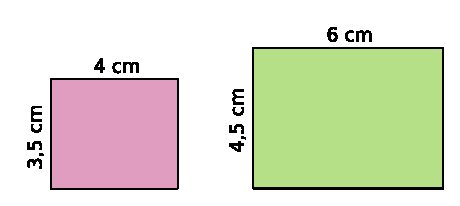
\includegraphics[width=7.4cm]{rectangles_rv} \end{center}
Les dimensions du premier rectangle sont‑elles proportionnelles aux dimensions du second rectangle ? Justifie ta réponse.
\end{exercice}


\begin{exercice}[Carré]
\begin{enumerate}
 \item Calcule le périmètre d'un carré de côté 3 cm.
 \item Le périmètre d'un carré est‑il proportionnel à la longueur du côté de ce carré ? Explique.
 \end{enumerate}
\end{exercice}


\begin{exercice}
Un cinéma propose les tarifs suivants :
 \begin{center}
  \begin{tabularx}{\linewidth}{|c|*{3}{>{\centering\arraybackslash}X|}}
  \hline
  Nombre de séances & 1 & 4 & 12 \\\hline
  Prix à payer (en CHF) & 12 & 48 & 135 \\\hline
 \end{tabularx}
\end{center}
Le prix est-il proportionnel au nombre de séances ?
\end{exercice}

%%%%%%%%%%%%%%%%%%%%%%%%%%%%%%%%%%%%%%%%%%%%%%%%%%%%%%%%%%%%%%%%%%%%%%%%

\serie{Compléter un tableau de proportionnalité}

\begin{exercice}
Recopie et complète les tableaux de proportionnalité :
\begin{enumerate}
 \item 
 
 \begin{minipage}[c]{0.18\linewidth}
 
\includegraphics[width=1.9cm]{bulle_mult6} 
  \end{minipage} \hfill
   \begin{minipage}[c]{0.76\linewidth}
   \begin{center}
 \renewcommand*\tabularxcolumn[1]{>{\centering\arraybackslash}m{#1}}
 \begin{ttableau}{\linewidth}{4}
 \hline
 \rowcolor{G2} 3 & 4 & 7,5 & \\\hline
 \rowcolor{D2} & & & 54 \\\hline
 \end{ttableau}
\end{center}
    \end{minipage} \\
\vspace{0.5cm}
 \item 
 
 \begin{minipage}[c]{0.18\linewidth}
 
\includegraphics[width=1.9cm]{bulle_mult12} 
  \end{minipage} \hfill
   \begin{minipage}[c]{0.76\linewidth}
   \begin{center}
 \renewcommand*\tabularxcolumn[1]{>{\centering\arraybackslash}m{#1}}
 \begin{ttableau}{\linewidth}{4}
 \hline
 \rowcolor{G2} 4 & 5,6 & & 15 \\\hline
 \rowcolor{D2} & & 12 & \\\hline
 \end{ttableau}
\end{center}
    \end{minipage} \\
 \end{enumerate}
\end{exercice}


\begin{exercice}
Recopie et complète les tableaux de proportionnalité :
\begin{enumerate}
 \item 
 
 \begin{minipage}[c]{0.18\linewidth}
 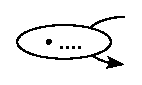
\includegraphics[width=1.9cm]{bulle_points} 
  \end{minipage} \hfill
   \begin{minipage}[c]{0.76\linewidth}
   \begin{center}
 \renewcommand*\tabularxcolumn[1]{>{\centering\arraybackslash}m{#1}}
 \begin{ttableau}{\linewidth}{4}
 \hline
 \rowcolor{G2} & 6 & 7 & 12,5 \\\hline
 \rowcolor{D2} 45 & & 35 & \\\hline
 \end{ttableau}
\end{center}
    \end{minipage} \\
\vspace{0.5cm}
 \item 
 
 \begin{minipage}[c]{0.18\linewidth}
 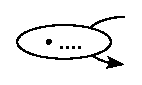
\includegraphics[width=1.9cm]{bulle_points} 
  \end{minipage} \hfill
   \begin{minipage}[c]{0.76\linewidth}
   \begin{center}
 \renewcommand*\tabularxcolumn[1]{>{\centering\arraybackslash}m{#1}}
 \begin{ttableau}{\linewidth}{4}
 \hline
 \rowcolor{G2} 6 & 5 & & 8,5 \\\hline
 \rowcolor{D2} 1,8 & & 1,2 & \\\hline
 \end{ttableau}
\end{center}
    \end{minipage} \\
 \end{enumerate}
\end{exercice}


\begin{exercice}
Recopie et complète les tableaux de proportionnalité suivants : \\[0.3em]
\begin{enumerate}
 \item 
 
\begin{center}
 \renewcommand*\tabularxcolumn[1]{>{\centering\arraybackslash}m{#1}}
 \begin{ttableau}{\linewidth}{6}
 \hline
 \rowcolor{C3} 0,2 & 0,4 & 0,6 & 0,8 & 6 & 14 \\\hline
 \rowcolor{F3} 6,5 & & 19,5 & & &  \\\hline
 \end{ttableau}
\end{center}
\vspace{0.3cm}
 \item 
 
\begin{center}
 \renewcommand*\tabularxcolumn[1]{>{\centering\arraybackslash}m{#1}}
 \begin{ttableau}{\linewidth}{6}
 \hline
 \rowcolor{C3} 4 & 2 & 1,8 & 5,8 & 0,4 & 6,2 \\\hline
 \rowcolor{F3} 9 & & 4,05 & & &  \\\hline
 \end{ttableau}
\end{center}
\vspace{0.3cm}
 \item 
 
\begin{center}
 \renewcommand*\tabularxcolumn[1]{>{\centering\arraybackslash}m{#1}}
 \begin{ttableau}{\linewidth}{6}
 \hline
 \rowcolor{C3} 3 & 6 & 1,5 & 4,5 & 18 & 22,5 \\\hline
 \rowcolor{F3} 4 & & & & &  \\\hline
 \end{ttableau}
\end{center}
\vspace{0.3cm}
 \item 
 
\begin{center}
 \renewcommand*\tabularxcolumn[1]{>{\centering\arraybackslash}m{#1}}
 \begin{ttableau}{\linewidth}{6}
 \hline
 \rowcolor{C3} 0,4 & 4 & 0,2 & 4,2 & 1,2 & 14 \\\hline
 \rowcolor{F3} 17 & & & & &  \\\hline
 \end{ttableau}
\end{center}
\end{enumerate}
\end{exercice}


\begin{exercice}[Jus de pomme]
Pour fabriquer 6 l de jus de pomme, on utilise 10 kg de pommes. Recopie et complète le tableau :
 \begin{center}
  \begin{tabularx}{\linewidth}{|c|*{3}{>{\centering\arraybackslash}X|}}
  \hline
 \rowcolor{J2} Quantité de pommes (en kg) & 10 & 7 & \\\hline
 \rowcolor{H2} Quantité de jus de pomme (en l) & & & 1 \\\hline
 \end{tabularx}
\end{center}
\end{exercice}


\begin{exercice}[Vitesse]
Un automobiliste, roulant à vitesse constante, parcourt 85 km en 1 h. Recopie et complète le tableau :
 \begin{center}
  \begin{tabularx}{\linewidth}{|c|*{3}{>{\centering\arraybackslash}X|}}
  \hline
 \rowcolor{J2} Distance parcourue (en km) & & 255 & \\\hline
 \rowcolor{H2} Durée (en h) & 1 & & 2,5 \\\hline
 \end{tabularx}
\end{center}
\end{exercice}


\begin{exercice}[À la cantine]
Dans une cantine scolaire, la masse de viande utilisée chaque jour est proportionnelle au nombre de repas préparés. Pour la préparation de 20 repas, 4 kg de viande sont utilisés. \\[0.5em]
Recopie et complète le tableau :
 \begin{center}
  \begin{tabularx}{\linewidth}{|c|*{3}{>{\centering\arraybackslash}X|}}
  \hline
 \rowcolor{J2} Nombre de repas & 20 & 150 & \\\hline
 \rowcolor{H2} Quantité de viande (en kg) & & & 10 \\\hline
 \end{tabularx}
\end{center}
\end{exercice}


\begin{exercice}
Les tableaux suivants sont des tableaux de proportionnalité. Recopie puis complète-les par la méthode de ton choix :
\begin{enumerate}
 \item 
 
\begin{center}
 \renewcommand*\tabularxcolumn[1]{>{\centering\arraybackslash}m{#1}}
 \begin{ttableau}{\linewidth}{5}
 \hline
 \rowcolor{H3} 2 & 5 & & 20 & \\\hline
 \rowcolor{F3} 5 & & 15 & & 60 \\\hline
 \end{ttableau}
\end{center}
\vspace{0.3cm}
 \item 
 
\begin{center}
 \renewcommand*\tabularxcolumn[1]{>{\centering\arraybackslash}m{#1}}
 \begin{ttableau}{\linewidth}{5}
 \hline
 \rowcolor{H3} 4 & 6 & & & 48 \\\hline
 \rowcolor{F3} 3 & & 12 & 36 & \\\hline
 \end{ttableau}
\end{center}
\end{enumerate}
\end{exercice}


\begin{exercice}
Un carton de 6 bouteilles de vin coûte 16,20 CHF. Recopie puis complète le tableau de proportionnalité suivant :
 \begin{center}
  \begin{tabularx}{\linewidth}{|c|*{3}{>{\centering\arraybackslash}X|}}
  \hline
 \rowcolor{U1} Nombre de bouteilles & 6 & 4 & \\\hline
 \rowcolor{H2} Prix (en CHF) & 16,2 & & 24,3 \\\hline
 \end{tabularx}
\end{center}
\end{exercice}


\begin{exercice}
Sur l’étiquette d’une bouteille d’un litre de jus de fruits, on lit :
\begin{center}
 \renewcommand*\tabularxcolumn[1]{>{\centering\arraybackslash}m{#1}}
 \begin{ttableau}{0.8\linewidth}{1}
\hline
Valeurs nutritionnelles moyennes \\ 
Protéines \qquad 0,4 g / 100 ml \\
Glucides \qquad 11,8 g / 100 ml \\
Lipides \qquad 0,1 g / 100 ml \\
Valeur énergétique moyenne : 50 Kcal \\\hline
\end{ttableau}
\end{center}
Recopie puis complète le tableau suivant :
 \begin{center}
  \begin{tabularx}{\linewidth}{|c|*{4}{>{\centering\arraybackslash}X|}}
  \hline
 Volume de jus d’orange & 1 l & 0,25 l & 1,5 l & 2 l \\\hline
 Protéines & & & &\\\hline
 Glucides & & & &\\\hline
 Lipides & & & &\\\hline
 Valeur énergétique & & & &\\\hline
 \end{tabularx}
\end{center}
\end{exercice}


\begin{exercice}
Pour préparer du foie gras, on doit préalablement saupoudrer le foie frais d'un mélange de sel et de poivre. Ce mélange doit être élaboré selon les proportions suivantes : une dose de poivre pour trois doses de sel. \\[0.5em]
Recopie puis complète le tableau suivant :
 \begin{center}
  \begin{tabularx}{\linewidth}{|c|*{6}{>{\centering\arraybackslash}X|}}
  \hline
 \rowcolor{D3} Poivre (en g) & 10 & & & 35 & & \\\hline
 \rowcolor{U1} Sel (en g) & & 60 & 36 & & 90 & 75 \\\hline
 \end{tabularx}
\end{center}
\end{exercice}

%%%%%%%%%%%%%%%%%%%%%%%%%%%%%%%%%%%%%%%%%%%%%%%%%%%%%%%%%%%%%%%%%%%%%%%%

\serie{Problèmes}

\begin{exercice}[À la braderie]
Lors d'une braderie, un disquaire vend tous les CDs au même prix. Pour deux CDs, Nicolas a payé 13,50 CHF. \\[0.5em]
Trace un tableau de proportionnalité et réponds :
\begin{enumerate}
 \item Quel prix Caroline va‑t‑elle payer si elle achète quatre CDs ?
 \item Quel prix Patrick va‑t‑il payer s'il achète trois CDs ?
 \item Anne a payé 47,25 CHF. Combien de CDs a‑t‑elle achetés ?
 \end{enumerate}
\end{exercice}


\begin{exercice}[À la laiterie]
Dans une laiterie, on utilise 19,6 l de lait pour fabriquer 3,5 kg de fromage. \\[0.5em]
Trace un tableau de proportionnalité et réponds :
\begin{enumerate}
 \item Quelle est la quantité de lait nécessaire à la fabrication de 5 kg de fromage ?
 \item Quelle quantité de fromage peut‑on fabriquer avec 70 l de lait ?
 \end{enumerate}
\end{exercice}


\begin{exercice}
Une moto consomme 4 l de carburant pour faire 100 km.
\begin{enumerate}
 \item Quelle est la consommation de cette moto pour faire 350 km ?
 \item Avec 9 l de carburant, quelle distance peut‑elle parcourir ?
 \end{enumerate}
\end{exercice}


\begin{exercice}[Recette]
Pour faire un gâteau pour six personnes, il faut 240 g de farine et 3 œufs. Quelle quantité de farine et combien d'œufs faut‑il pour faire ce gâteau pour quatre personnes ?
\end{exercice}


\begin{exercice}
Un robinet permet de remplir huit seaux de dix litres en trois minutes.
\begin{enumerate}
 \item Quel est le temps nécessaire pour remplir un réservoir de 480 l ?
 \item Quelle est la quantité d'eau écoulée en 15 min ?
 \item Si on laisse, par mégarde, ce robinet ouvert pendant deux heures, quelle sera la quantité d'eau écoulée ?
 \end{enumerate}
\end{exercice}


\begin{exercice}[Cuisson]
Un livre de cuisine indique que, pour faire cuire le rôti, il faut compter « 15 min à four chaud pour 500 g de viande ».
\begin{enumerate}
 \item Calcule le temps nécessaire à la cuisson d'un rôti pesant 750 g ;
 \item Même question avec un rôti pesant 600 g.
 \end{enumerate}
\end{exercice}


\begin{exercice}[Des baguettes]
Pour 4,25 CHF, j'ai acheté cinq baguettes de pain. Pour 5,95 CHF, j'aurais eu sept baguettes. Le prix payé est proportionnel au nombre de baguettes. \\[0.5em]
Sans calculer le prix d'une baguette, calcule :
\begin{enumerate}
 \item Le prix de douze baguettes ;
 \item Le prix de deux baguettes ;
 \item Le prix de trois baguettes ;
 \item Le prix de quinze baguettes.
 \end{enumerate}
\end{exercice}


\begin{exercice}
Pour obtenir un verre de sirop, on a versé 8 cl de grenadine dans 30 cl d’eau. \\[0.5em]
Quelle quantité de grenadine faut-il mettre dans 45 cl d’eau pour obtenir exactement le même goût ?
\end{exercice}


\begin{exercice}
Une chaîne d’embouteillage produit 1 200 bouteilles en 3 heures.
\begin{enumerate}
 \item Combien de bouteilles produit-elle en une heure ? En deux heures ?
 \item Combien de temps faut-il pour produire 6 000 bouteilles ?
 \end{enumerate}
\end{exercice}


\begin{exercice}
Pour remonter l'ancre de son voilier, un marin a mis 3 minutes pour enrouler 21 m de chaîne. Lors d’une autre escale, il a mis 4 min 30 s pour 31,50 m.
\begin{enumerate}
 \item En supposant qu'il le fasse à vitesse constante, combien de temps mettra-t-il pour remonter une ancre jetée à 10,50 m de fond ?
 \item Quelle longueur de chaîne enroulera-t-il en 13 min 30 s ?
 \end{enumerate}
\end{exercice}

%%%%%%%%%%%%%%%%%%%%%%%%%%%%%%%%%%%%%%%%%%%%%%%%%%%%%%%%%%%%%%%%%%%%%%%%

